% Options for packages loaded elsewhere
\PassOptionsToPackage{unicode}{hyperref}
\PassOptionsToPackage{hyphens}{url}
\PassOptionsToPackage{dvipsnames,svgnames,x11names}{xcolor}
%
\documentclass[
  letterpaper,
  DIV=11,
  numbers=noendperiod]{scrreprt}

\usepackage{amsmath,amssymb}
\usepackage{lmodern}
\usepackage{iftex}
\ifPDFTeX
  \usepackage[T1]{fontenc}
  \usepackage[utf8]{inputenc}
  \usepackage{textcomp} % provide euro and other symbols
\else % if luatex or xetex
  \usepackage{unicode-math}
  \defaultfontfeatures{Scale=MatchLowercase}
  \defaultfontfeatures[\rmfamily]{Ligatures=TeX,Scale=1}
\fi
% Use upquote if available, for straight quotes in verbatim environments
\IfFileExists{upquote.sty}{\usepackage{upquote}}{}
\IfFileExists{microtype.sty}{% use microtype if available
  \usepackage[]{microtype}
  \UseMicrotypeSet[protrusion]{basicmath} % disable protrusion for tt fonts
}{}
\makeatletter
\@ifundefined{KOMAClassName}{% if non-KOMA class
  \IfFileExists{parskip.sty}{%
    \usepackage{parskip}
  }{% else
    \setlength{\parindent}{0pt}
    \setlength{\parskip}{6pt plus 2pt minus 1pt}}
}{% if KOMA class
  \KOMAoptions{parskip=half}}
\makeatother
\usepackage{xcolor}
\setlength{\emergencystretch}{3em} % prevent overfull lines
\setcounter{secnumdepth}{5}
% Make \paragraph and \subparagraph free-standing
\ifx\paragraph\undefined\else
  \let\oldparagraph\paragraph
  \renewcommand{\paragraph}[1]{\oldparagraph{#1}\mbox{}}
\fi
\ifx\subparagraph\undefined\else
  \let\oldsubparagraph\subparagraph
  \renewcommand{\subparagraph}[1]{\oldsubparagraph{#1}\mbox{}}
\fi

\usepackage{color}
\usepackage{fancyvrb}
\newcommand{\VerbBar}{|}
\newcommand{\VERB}{\Verb[commandchars=\\\{\}]}
\DefineVerbatimEnvironment{Highlighting}{Verbatim}{commandchars=\\\{\}}
% Add ',fontsize=\small' for more characters per line
\usepackage{framed}
\definecolor{shadecolor}{RGB}{241,243,245}
\newenvironment{Shaded}{\begin{snugshade}}{\end{snugshade}}
\newcommand{\AlertTok}[1]{\textcolor[rgb]{0.68,0.00,0.00}{#1}}
\newcommand{\AnnotationTok}[1]{\textcolor[rgb]{0.37,0.37,0.37}{#1}}
\newcommand{\AttributeTok}[1]{\textcolor[rgb]{0.40,0.45,0.13}{#1}}
\newcommand{\BaseNTok}[1]{\textcolor[rgb]{0.68,0.00,0.00}{#1}}
\newcommand{\BuiltInTok}[1]{\textcolor[rgb]{0.00,0.23,0.31}{#1}}
\newcommand{\CharTok}[1]{\textcolor[rgb]{0.13,0.47,0.30}{#1}}
\newcommand{\CommentTok}[1]{\textcolor[rgb]{0.37,0.37,0.37}{#1}}
\newcommand{\CommentVarTok}[1]{\textcolor[rgb]{0.37,0.37,0.37}{\textit{#1}}}
\newcommand{\ConstantTok}[1]{\textcolor[rgb]{0.56,0.35,0.01}{#1}}
\newcommand{\ControlFlowTok}[1]{\textcolor[rgb]{0.00,0.23,0.31}{#1}}
\newcommand{\DataTypeTok}[1]{\textcolor[rgb]{0.68,0.00,0.00}{#1}}
\newcommand{\DecValTok}[1]{\textcolor[rgb]{0.68,0.00,0.00}{#1}}
\newcommand{\DocumentationTok}[1]{\textcolor[rgb]{0.37,0.37,0.37}{\textit{#1}}}
\newcommand{\ErrorTok}[1]{\textcolor[rgb]{0.68,0.00,0.00}{#1}}
\newcommand{\ExtensionTok}[1]{\textcolor[rgb]{0.00,0.23,0.31}{#1}}
\newcommand{\FloatTok}[1]{\textcolor[rgb]{0.68,0.00,0.00}{#1}}
\newcommand{\FunctionTok}[1]{\textcolor[rgb]{0.28,0.35,0.67}{#1}}
\newcommand{\ImportTok}[1]{\textcolor[rgb]{0.00,0.46,0.62}{#1}}
\newcommand{\InformationTok}[1]{\textcolor[rgb]{0.37,0.37,0.37}{#1}}
\newcommand{\KeywordTok}[1]{\textcolor[rgb]{0.00,0.23,0.31}{#1}}
\newcommand{\NormalTok}[1]{\textcolor[rgb]{0.00,0.23,0.31}{#1}}
\newcommand{\OperatorTok}[1]{\textcolor[rgb]{0.37,0.37,0.37}{#1}}
\newcommand{\OtherTok}[1]{\textcolor[rgb]{0.00,0.23,0.31}{#1}}
\newcommand{\PreprocessorTok}[1]{\textcolor[rgb]{0.68,0.00,0.00}{#1}}
\newcommand{\RegionMarkerTok}[1]{\textcolor[rgb]{0.00,0.23,0.31}{#1}}
\newcommand{\SpecialCharTok}[1]{\textcolor[rgb]{0.37,0.37,0.37}{#1}}
\newcommand{\SpecialStringTok}[1]{\textcolor[rgb]{0.13,0.47,0.30}{#1}}
\newcommand{\StringTok}[1]{\textcolor[rgb]{0.13,0.47,0.30}{#1}}
\newcommand{\VariableTok}[1]{\textcolor[rgb]{0.07,0.07,0.07}{#1}}
\newcommand{\VerbatimStringTok}[1]{\textcolor[rgb]{0.13,0.47,0.30}{#1}}
\newcommand{\WarningTok}[1]{\textcolor[rgb]{0.37,0.37,0.37}{\textit{#1}}}

\providecommand{\tightlist}{%
  \setlength{\itemsep}{0pt}\setlength{\parskip}{0pt}}\usepackage{longtable,booktabs,array}
\usepackage{calc} % for calculating minipage widths
% Correct order of tables after \paragraph or \subparagraph
\usepackage{etoolbox}
\makeatletter
\patchcmd\longtable{\par}{\if@noskipsec\mbox{}\fi\par}{}{}
\makeatother
% Allow footnotes in longtable head/foot
\IfFileExists{footnotehyper.sty}{\usepackage{footnotehyper}}{\usepackage{footnote}}
\makesavenoteenv{longtable}
\usepackage{graphicx}
\makeatletter
\def\maxwidth{\ifdim\Gin@nat@width>\linewidth\linewidth\else\Gin@nat@width\fi}
\def\maxheight{\ifdim\Gin@nat@height>\textheight\textheight\else\Gin@nat@height\fi}
\makeatother
% Scale images if necessary, so that they will not overflow the page
% margins by default, and it is still possible to overwrite the defaults
% using explicit options in \includegraphics[width, height, ...]{}
\setkeys{Gin}{width=\maxwidth,height=\maxheight,keepaspectratio}
% Set default figure placement to htbp
\makeatletter
\def\fps@figure{htbp}
\makeatother
\newlength{\cslhangindent}
\setlength{\cslhangindent}{1.5em}
\newlength{\csllabelwidth}
\setlength{\csllabelwidth}{3em}
\newlength{\cslentryspacingunit} % times entry-spacing
\setlength{\cslentryspacingunit}{\parskip}
\newenvironment{CSLReferences}[2] % #1 hanging-ident, #2 entry spacing
 {% don't indent paragraphs
  \setlength{\parindent}{0pt}
  % turn on hanging indent if param 1 is 1
  \ifodd #1
  \let\oldpar\par
  \def\par{\hangindent=\cslhangindent\oldpar}
  \fi
  % set entry spacing
  \setlength{\parskip}{#2\cslentryspacingunit}
 }%
 {}
\usepackage{calc}
\newcommand{\CSLBlock}[1]{#1\hfill\break}
\newcommand{\CSLLeftMargin}[1]{\parbox[t]{\csllabelwidth}{#1}}
\newcommand{\CSLRightInline}[1]{\parbox[t]{\linewidth - \csllabelwidth}{#1}\break}
\newcommand{\CSLIndent}[1]{\hspace{\cslhangindent}#1}

\usepackage{booktabs}
\usepackage{longtable}
\usepackage{array}
\usepackage{multirow}
\usepackage{wrapfig}
\usepackage{float}
\usepackage{colortbl}
\usepackage{pdflscape}
\usepackage{tabu}
\usepackage{threeparttable}
\usepackage{threeparttablex}
\usepackage[normalem]{ulem}
\usepackage{makecell}
\usepackage{xcolor}
\usepackage{amsmath}
\usepackage{caption}
\KOMAoption{captions}{tableheading}
\makeatletter
\makeatother
\makeatletter
\@ifpackageloaded{bookmark}{}{\usepackage{bookmark}}
\makeatother
\makeatletter
\@ifpackageloaded{caption}{}{\usepackage{caption}}
\AtBeginDocument{%
\ifdefined\contentsname
  \renewcommand*\contentsname{Table of contents}
\else
  \newcommand\contentsname{Table of contents}
\fi
\ifdefined\listfigurename
  \renewcommand*\listfigurename{List of Figures}
\else
  \newcommand\listfigurename{List of Figures}
\fi
\ifdefined\listtablename
  \renewcommand*\listtablename{List of Tables}
\else
  \newcommand\listtablename{List of Tables}
\fi
\ifdefined\figurename
  \renewcommand*\figurename{Figure}
\else
  \newcommand\figurename{Figure}
\fi
\ifdefined\tablename
  \renewcommand*\tablename{Table}
\else
  \newcommand\tablename{Table}
\fi
}
\@ifpackageloaded{float}{}{\usepackage{float}}
\floatstyle{ruled}
\@ifundefined{c@chapter}{\newfloat{codelisting}{h}{lop}}{\newfloat{codelisting}{h}{lop}[chapter]}
\floatname{codelisting}{Listing}
\newcommand*\listoflistings{\listof{codelisting}{List of Listings}}
\makeatother
\makeatletter
\@ifpackageloaded{caption}{}{\usepackage{caption}}
\@ifpackageloaded{subcaption}{}{\usepackage{subcaption}}
\makeatother
\makeatletter
\@ifpackageloaded{tcolorbox}{}{\usepackage[many]{tcolorbox}}
\makeatother
\makeatletter
\@ifundefined{shadecolor}{\definecolor{shadecolor}{rgb}{.97, .97, .97}}
\makeatother
\makeatletter
\makeatother
\ifLuaTeX
  \usepackage{selnolig}  % disable illegal ligatures
\fi
\IfFileExists{bookmark.sty}{\usepackage{bookmark}}{\usepackage{hyperref}}
\IfFileExists{xurl.sty}{\usepackage{xurl}}{} % add URL line breaks if available
\urlstyle{same} % disable monospaced font for URLs
\hypersetup{
  pdftitle={PREGVAL Book},
  pdfauthor={Francisco Sanchez-Saez},
  colorlinks=true,
  linkcolor={blue},
  filecolor={Maroon},
  citecolor={Blue},
  urlcolor={Blue},
  pdfcreator={LaTeX via pandoc}}

\title{PREGVAL Book}
\author{Francisco Sanchez-Saez}
\date{6/6/23}

\begin{document}
\maketitle
\ifdefined\Shaded\renewenvironment{Shaded}{\begin{tcolorbox}[breakable, interior hidden, boxrule=0pt, borderline west={3pt}{0pt}{shadecolor}, enhanced, frame hidden, sharp corners]}{\end{tcolorbox}}\fi

\renewcommand*\contentsname{Table of contents}
{
\hypersetup{linkcolor=}
\setcounter{tocdepth}{2}
\tableofcontents
}
\bookmarksetup{startatroot}

\hypertarget{preface}{%
\chapter*{Preface}\label{preface}}
\addcontentsline{toc}{chapter}{Preface}

\markboth{Preface}{Preface}

This is a Quarto book.

To learn more about Quarto books visit
\url{https://quarto.org/docs/books}.

\begin{Shaded}
\begin{Highlighting}[]
\DecValTok{1} \SpecialCharTok{+} \DecValTok{1}
\end{Highlighting}
\end{Shaded}

\begin{verbatim}
[1] 2
\end{verbatim}

\bookmarksetup{startatroot}

\hypertarget{introduction}{%
\chapter{Introduction}\label{introduction}}

This is a book created from markdown and executable code.

See Knuth (1984) for additional discussion of literate programming.

\begin{Shaded}
\begin{Highlighting}[]
\DecValTok{1} \SpecialCharTok{+} \DecValTok{1}
\end{Highlighting}
\end{Shaded}

\begin{verbatim}
[1] 2
\end{verbatim}

\bookmarksetup{startatroot}

\hypertarget{quality-check-processing-mbds}{%
\chapter{Quality Check: Processing
MBDS}\label{quality-check-processing-mbds}}

The table to be analysed is \textbf{mbds\_2009\_2012\_clean.csv}.

\bookmarksetup{startatroot}

\hypertarget{check-variables}{%
\chapter{Check variables}\label{check-variables}}

The variables extracted from mbds are:
\textcolor{blue}{sip, fecha_ingreso, fecha_alta, dpto_cod, hosp_cod, serv_ing_cod, serv_ing_desc, tipo_activ, circ_ing_cod, circ_ing_desc, circ_alta_cod, circ_alta_desc, d1, d2, d3, d4, d5, d6, d7, d8, d9, d10, d11, d12, d13, d14, d15, d16, d17, d18, d19, d20, d21, d22, d23, d24, d25, d26, d27, d28, d29, d30, p1, p2, p3, p4, p5, p6, p7, p8, p9, p10, p11, p12, p13, p14, p15, p16, p17, p18, p19, p20, p21, p22, p23, p24, p25, p26, p27, p28, p29, p30, tipo_codigo, fecha_parto, parto_multiple, semana_gest, peso1, sexo1, peso2, sexo2, peso3, sexo3, ind_uci, and estancias_uci}.

\hypertarget{check-mandatory-vars}{%
\section{Check mandatory vars}\label{check-mandatory-vars}}

\textcolor{green}{All mandatory vars are present}.

\hypertarget{check-all-vars}{%
\section{Check all vars}\label{check-all-vars}}

\textcolor{red}{dpto_desc and hosp_desc were not extracted}.

\hypertarget{completeness}{%
\section{Completeness}\label{completeness}}

In Figure~\ref{fig-completeness} is shown the percentage of non-missing
values for each variable. Non-mandatory variables are shown at the
bottom of the figure.

\begin{figure}

{\centering \includegraphics[width=31.25in,height=\textheight]{./04_MBDS_QC_2009_2012_files/figure-pdf/fig-completeness-1.pdf}

}

\caption{\label{fig-completeness}Variables completeness}

\end{figure}

\bookmarksetup{startatroot}

\hypertarget{check-content}{%
\chapter{Check content}\label{check-content}}

The \textbf{mbds} table has a total of \textbf{n = 100 observations}.

\hypertarget{population}{%
\section{Population}\label{population}}

\begin{itemize}
\tightlist
\item
  In \textbf{mbds} table there are \textcolor{blue}{100} distinct
  individuals.
  \textcolor{green}{All the individuals are included in the target population}.
  Therefore, there are \textcolor{green}{100} individuals included in
  the target population out of the
  \textcolor{purple}{3&#x200A;&#x200D;655&#x200A;&#x200D;656} total
  individuals in the cohort. These represents
  \textbackslash textcolor\{blue\}\{0\%\} of the total.
\end{itemize}

\begin{itemize}
\tightlist
\item
  The Table~\ref{tbl-sipsperyear} shows the number of individuals per
  year of the study period.
\end{itemize}

\hypertarget{tbl-sipsperyear}{}
\begin{longtable}{cc}
\caption{\label{tbl-sipsperyear}Number of individuals per year of calculation }\tabularnewline

\toprule
Year of admission & Count of distinct individuals \\ 
\midrule
2010 & 100 \\ 
\bottomrule
\end{longtable}

\hypertarget{date-of-the-admission}{%
\section{Date of the admission}\label{date-of-the-admission}}

The variable \emph{fecha\_ingreso} is missing in \textbf{0
observations}, so it is \textbackslash textcolor\{green\}\{100\%\}
complete. The minimum and maximum date are \textbf{\emph{2010-01-03}}
and \textbf{\emph{2010-12-28}} respectively. Table~\ref{tbl-fechaing}
shows the number of admissions per year of \emph{fecha\_ingreso}.

\textcolor{green}{All dates are inside the study period}.

\hypertarget{tbl-fechaing}{}
\begin{longtable}{ll}
\caption{\label{tbl-fechaing}Number of admissions each year of calculation }\tabularnewline

\toprule
Year of the admission & Count \\ 
\midrule
2010 & 100 \\ 
\bottomrule
\end{longtable}

The month and year with less admissions was
\textcolor{blue}{April 2010 with n = 5},
\textcolor{blue}{July 2010 with n = 5} and the month and year with more
admissions was \textcolor{purple}{November 2010 with n = 14}.

In Figure~\ref{fig-ingresoyear}, Figure~\ref{fig-ingresomonth}, and
Figure~\ref{fig-ingresoday} are presented the frequencies of years,
months, and days of the admissions respectively.

\begin{figure}

{\centering \includegraphics[width=31.25in,height=\textheight]{./04_MBDS_QC_2009_2012_files/figure-pdf/fig-ingresoyear-1.pdf}

}

\caption{\label{fig-ingresoyear}Admission year}

\end{figure}

\begin{figure}

{\centering \includegraphics[width=31.25in,height=\textheight]{./04_MBDS_QC_2009_2012_files/figure-pdf/fig-ingresomonth-1.pdf}

}

\caption{\label{fig-ingresomonth}Admission month}

\end{figure}

\begin{figure}

{\centering \includegraphics[width=31.25in,height=\textheight]{./04_MBDS_QC_2009_2012_files/figure-pdf/fig-ingresoday-1.pdf}

}

\caption{\label{fig-ingresoday}Admission day}

\end{figure}

\hypertarget{date-of-the-discharge}{%
\section{Date of the discharge}\label{date-of-the-discharge}}

The variable \emph{fecha\_alta} is missing in \textbf{0 observations},
so it is \textbackslash textcolor\{green\}\{100\%\} complete. The
minimum and maximum date are \textbf{\emph{2010-01-04}} and
\textbf{\emph{2010-12-30}} respectively. Table~\ref{tbl-fechaalta} shows
the number of discharges per year of \emph{fecha\_alta}.

\textcolor{green}{All dates are inside the study period}.

\hypertarget{tbl-fechaalta}{}
\begin{longtable}{ll}
\caption{\label{tbl-fechaalta}Number of discharges each year of calculation }\tabularnewline

\toprule
Year of the discharge & Count \\ 
\midrule
2010 & 100 \\ 
\bottomrule
\end{longtable}

The month and year with less discharges was
\textcolor{blue}{January 2010 with n = 6},
\textcolor{blue}{April 2010 with n = 6},
\textcolor{blue}{July 2010 with n = 6},
\textcolor{blue}{September 2010 with n = 6} and the month and year with
more discharges was \textcolor{purple}{November 2010 with n = 14}.

In Figure~\ref{fig-altayear}, Figure~\ref{fig-altamonth}, and
Figure~\ref{fig-altaday} are presented the frequencies of years, months,
and days of the visits respectively.

\begin{figure}

{\centering \includegraphics[width=31.25in,height=\textheight]{./04_MBDS_QC_2009_2012_files/figure-pdf/fig-altayear-1.pdf}

}

\caption{\label{fig-altayear}Discharge year}

\end{figure}

\begin{figure}

{\centering \includegraphics[width=31.25in,height=\textheight]{./04_MBDS_QC_2009_2012_files/figure-pdf/fig-altamonth-1.pdf}

}

\caption{\label{fig-altamonth}Discharge month}

\end{figure}

\begin{figure}

{\centering \includegraphics[width=31.25in,height=\textheight]{./04_MBDS_QC_2009_2012_files/figure-pdf/fig-altaday-1.pdf}

}

\caption{\label{fig-altaday}Discharge day}

\end{figure}

\hypertarget{visit-service}{%
\section{Visit service}\label{visit-service}}

The variable \emph{serv\_ing\_desc} is missing in \textbf{1
observations}, so it is \textbackslash textcolor\{orange\}\{99\%\}
complete. Table~\ref{tbl-visit} shows all the services used in the
primary care visits arranged by alphabetic order. Figure~\ref{fig-serv}
shows the count of the utilization of each visit service. Finally,
Figure~\ref{fig-servyear} shows the count of visits for the 10 most used
services per year.

\hypertarget{tbl-visit}{}
\begin{longtable}{llll}
\caption{\label{tbl-visit}Healths services used in the primary care visits }\tabularnewline

\toprule
Service & Count & Percentage & valid\_percent \\ 
\midrule
CARDIOLOGIA & 2 & 2.00\% & 2.02\% \\ 
CIRUGIA GENERAL & 10 & 10.00\% & 10.10\% \\ 
CIRUGIA GENERAL Y DIGESTIVO & 3 & 3.00\% & 3.03\% \\ 
CIRUGIA MAXILOFACIAL & 2 & 2.00\% & 2.02\% \\ 
CIRUGIA ORTOPEDICA Y TRAUMATOLOGÍA & 5 & 5.00\% & 5.05\% \\ 
CIRUGIA PLASTICA & 1 & 1.00\% & 1.01\% \\ 
DERMATOLOGIA & 2 & 2.00\% & 2.02\% \\ 
GINECOLOGIA & 16 & 16.00\% & 16.16\% \\ 
HEMATOLOGIA & 1 & 1.00\% & 1.01\% \\ 
MEDICINA DIGESTIVA & 1 & 1.00\% & 1.01\% \\ 
MEDICINA INTERNA & 3 & 3.00\% & 3.03\% \\ 
NEFROLOGIA & 1 & 1.00\% & 1.01\% \\ 
NEUMOLOGIA & 2 & 2.00\% & 2.02\% \\ 
NEUROCIRUGIA & 2 & 2.00\% & 2.02\% \\ 
NEUROFISIOLOGIA & 1 & 1.00\% & 1.01\% \\ 
OBSTETRICIA & 33 & 33.00\% & 33.33\% \\ 
OTORRINOLARINGOLOGIA & 2 & 2.00\% & 2.02\% \\ 
PEDIATRIA & 1 & 1.00\% & 1.01\% \\ 
PSIQUIATRIA & 1 & 1.00\% & 1.01\% \\ 
REPRODUCCION & 1 & 1.00\% & 1.01\% \\ 
REUMATOLOGIA & 1 & 1.00\% & 1.01\% \\ 
UNIDAD CORTA ESTANCIA & 1 & 1.00\% & 1.01\% \\ 
UNIDAD ENFERMEDADES INFECCIOSAS & 1 & 1.00\% & 1.01\% \\ 
UNIDAD TRANSTORNOS ALIMENTARIOS & 1 & 1.00\% & 1.01\% \\ 
UROLOGIA & 5 & 5.00\% & 5.05\% \\ 
NA & 1 & 1.00\% & - \\ 
\bottomrule
\end{longtable}

\begin{figure}

{\centering \includegraphics[width=31.25in,height=\textheight]{./04_MBDS_QC_2009_2012_files/figure-pdf/fig-serv-1.pdf}

}

\caption{\label{fig-serv}Primary care visit services}

\end{figure}

\begin{figure}

{\centering \includegraphics[width=31.25in,height=\textheight]{./04_MBDS_QC_2009_2012_files/figure-pdf/fig-servyear-1.pdf}

}

\caption{\label{fig-servyear}Most used primary care visit services per
year}

\end{figure}

\hypertarget{diagnoses-codes}{%
\section{Diagnoses codes}\label{diagnoses-codes}}

The variable \emph{d1} is missing in \textbf{0 observations}, so it is
\textbackslash textcolor\{green\}\{100\%\} complete.
Figure~\ref{fig-code} shows the most employed diagnoses codes. Finally,
Figure~\ref{fig-codeyear} shows the count of the 10 most employed codes
per year.

\begin{figure}

{\centering \includegraphics[width=31.25in,height=\textheight]{./04_MBDS_QC_2009_2012_files/figure-pdf/fig-code-1.pdf}

}

\caption{\label{fig-code}Diagnosis codes used in primary care visits}

\end{figure}

\begin{verbatim}
#> Warning: ggrepel: 69 unlabeled data points (too many overlaps). Consider
#> increasing max.overlaps
\end{verbatim}

\begin{figure}

{\centering \includegraphics[width=31.25in,height=\textheight]{./04_MBDS_QC_2009_2012_files/figure-pdf/fig-codeyear-1.pdf}

}

\caption{\label{fig-codeyear}Diagnosis codes used in primary care visits
per year}

\end{figure}

\hypertarget{code-vocabulary}{%
\section{Code vocabulary}\label{code-vocabulary}}

The variable \emph{tipo\_codigo} is missing in \textbf{0 observations},
so it is \textbackslash textcolor\{green\}\{100\%\} complete.
Figure~\ref{fig-tipo} shows the count of the utilization of each visit
service. Finally, Figure~\ref{fig-tipoyear} shows the count of visits
for the 10 most used services per year.

\begin{figure}

{\centering \includegraphics[width=31.25in,height=\textheight]{./04_MBDS_QC_2009_2012_files/figure-pdf/fig-tipo-1.pdf}

}

\caption{\label{fig-tipo}Code vocabularies used in primary care visits}

\end{figure}

\begin{figure}

{\centering \includegraphics[width=31.25in,height=\textheight]{./04_MBDS_QC_2009_2012_files/figure-pdf/fig-tipoyear-1.pdf}

}

\caption{\label{fig-tipoyear}Code vocabularies used in primary care
visits per year}

\end{figure}

\hypertarget{date-of-the-labour}{%
\section{Date of the labour}\label{date-of-the-labour}}

The variable \emph{fecha\_parto} is missing in \textbf{86 observations},
so it is \textbackslash textcolor\{orange\}\{14\%\} complete. The
minimum and maximum date are \textbf{\emph{2010-01-27}} and
\textbf{\emph{2010-12-09}} respectively. Table~\ref{tbl-fechaparto}
shows the number of discharges per year of \emph{fecha\_parto}.

\textcolor{green}{All dates are inside the study period}.

\hypertarget{tbl-fechaparto}{}
\begin{longtable}{ll}
\caption{\label{tbl-fechaparto}Number of discharges each year of calculation }\tabularnewline

\toprule
Year of the labour & Count \\ 
\midrule
2010 & 14 \\ 
NA & 86 \\ 
\bottomrule
\end{longtable}

The month and year with less labours was
\textcolor{blue}{January 2010 with n = 1},
\textcolor{blue}{June 2010 with n = 1},
\textcolor{blue}{August 2010 with n = 1},
\textcolor{blue}{October 2010 with n = 1},
\textcolor{blue}{December 2010 with n = 1} and the month and year with
more labours was \textcolor{purple}{NA NA with n = 86}.

In Figure~\ref{fig-labouryear}, Figure~\ref{fig-labourmonth}, and
Figure~\ref{fig-labourday} are presented the frequencies of years,
months, and days of the visits respectively.

\begin{figure}

{\centering \includegraphics[width=31.25in,height=\textheight]{./04_MBDS_QC_2009_2012_files/figure-pdf/fig-labouryear-1.pdf}

}

\caption{\label{fig-labouryear}Labour year}

\end{figure}

\begin{figure}

{\centering \includegraphics[width=31.25in,height=\textheight]{./04_MBDS_QC_2009_2012_files/figure-pdf/fig-labourmonth-1.pdf}

}

\caption{\label{fig-labourmonth}Labour month}

\end{figure}

\begin{figure}

{\centering \includegraphics[width=31.25in,height=\textheight]{./04_MBDS_QC_2009_2012_files/figure-pdf/fig-labourday-1.pdf}

}

\caption{\label{fig-labourday}Labour day}

\end{figure}

\bookmarksetup{startatroot}

\hypertarget{quality-check-processing-mbds-1}{%
\chapter{Quality Check: Processing
MBDS}\label{quality-check-processing-mbds-1}}

The table to be analysed is \textbf{mbds\_2018\_2021\_clean.csv}.

\bookmarksetup{startatroot}

\hypertarget{check-variables-1}{%
\chapter{Check variables}\label{check-variables-1}}

The variables extracted from mbds are:
\textcolor{blue}{sip, fecha_ingreso, fecha_alta, dpto_cod, hosp_cod, serv_ing_cod, serv_ing_desc, tipo_activ, circ_ing_cod, circ_ing_desc, circ_alta_cod, circ_alta_desc, d1, d2, d3, d4, d5, d6, d7, d8, d9, d10, d11, d12, d13, d14, d15, d16, d17, d18, d19, d20, d21, d22, d23, d24, d25, d26, d27, d28, d29, d30, p1, p2, p3, p4, p5, p6, p7, p8, p9, p10, p11, p12, p13, p14, p15, p16, p17, p18, p19, p20, p21, p22, p23, p24, p25, p26, p27, p28, p29, p30, tipo_codigo, fecha_parto, parto_multiple, semana_gest, peso1, sexo1, peso2, sexo2, peso3, sexo3, ind_uci, and estancias_uci}.

\hypertarget{check-mandatory-vars-1}{%
\section{Check mandatory vars}\label{check-mandatory-vars-1}}

\textcolor{green}{All mandatory vars are present}.

\hypertarget{check-all-vars-1}{%
\section{Check all vars}\label{check-all-vars-1}}

\textcolor{red}{dpto_desc and hosp_desc were not extracted}.

\hypertarget{completeness-1}{%
\section{Completeness}\label{completeness-1}}

In Figure~\ref{fig-completeness} is shown the percentage of non-missing
values for each variable. Non-mandatory variables are shown at the
bottom of the figure.

\begin{figure}

{\centering \includegraphics[width=31.25in,height=\textheight]{./04_MBDS_QC_2018_2021_files/figure-pdf/fig-completeness-1.pdf}

}

\caption{\label{fig-completeness}Variables completeness}

\end{figure}

\bookmarksetup{startatroot}

\hypertarget{check-content-1}{%
\chapter{Check content}\label{check-content-1}}

The \textbf{mbds} table has a total of \textbf{n = 100 observations}.

\hypertarget{population-1}{%
\section{Population}\label{population-1}}

\begin{itemize}
\tightlist
\item
  In \textbf{mbds} table there are \textcolor{blue}{100} distinct
  individuals.
  \textcolor{green}{All the individuals are included in the target population}.
  Therefore, there are \textcolor{green}{100} individuals included in
  the target population out of the
  \textcolor{purple}{3&#x200A;&#x200D;655&#x200A;&#x200D;656} total
  individuals in the cohort. These represents
  \textbackslash textcolor\{blue\}\{0\%\} of the total.
\end{itemize}

\begin{itemize}
\tightlist
\item
  The Table~\ref{tbl-sipsperyear} shows the number of individuals per
  year of the study period.
\end{itemize}

\hypertarget{tbl-sipsperyear}{}
\begin{longtable}{cc}
\caption{\label{tbl-sipsperyear}Number of individuals per year of calculation }\tabularnewline

\toprule
Year of admission & Count of distinct individuals \\ 
\midrule
2018 & 26 \\ 
2019 & 23 \\ 
2020 & 26 \\ 
2021 & 25 \\ 
\bottomrule
\end{longtable}

\hypertarget{date-of-the-admission-1}{%
\section{Date of the admission}\label{date-of-the-admission-1}}

The variable \emph{fecha\_ingreso} is missing in \textbf{0
observations}, so it is \textbackslash textcolor\{green\}\{100\%\}
complete. The minimum and maximum date are \textbf{\emph{2018-01-02}}
and \textbf{\emph{2021-12-20}} respectively. Table~\ref{tbl-fechaing}
shows the number of admissions per year of \emph{fecha\_ingreso}.

\textcolor{green}{All dates are inside the study period}.

\hypertarget{tbl-fechaing}{}
\begin{longtable}{ll}
\caption{\label{tbl-fechaing}Number of admissions each year of calculation }\tabularnewline

\toprule
Year of the admission & Count \\ 
\midrule
2018 & 26 \\ 
2019 & 23 \\ 
2020 & 26 \\ 
2021 & 25 \\ 
\bottomrule
\end{longtable}

The month and year with less admissions was
\textcolor{blue}{March 2018 with n = 1},
\textcolor{blue}{May 2018 with n = 1},
\textcolor{blue}{November 2018 with n = 1},
\textcolor{blue}{December 2018 with n = 1},
\textcolor{blue}{March 2019 with n = 1},
\textcolor{blue}{May 2019 with n = 1},
\textcolor{blue}{June 2019 with n = 1},
\textcolor{blue}{November 2019 with n = 1},
\textcolor{blue}{May 2020 with n = 1},
\textcolor{blue}{June 2020 with n = 1},
\textcolor{blue}{July 2020 with n = 1},
\textcolor{blue}{May 2021 with n = 1},
\textcolor{blue}{September 2021 with n = 1},
\textcolor{blue}{December 2021 with n = 1} and the month and year with
more admissions was \textcolor{purple}{April 2018 with n = 5},
\textcolor{purple}{July 2018 with n = 5}.

In Figure~\ref{fig-ingresoyear}, Figure~\ref{fig-ingresomonth}, and
Figure~\ref{fig-ingresoday} are presented the frequencies of years,
months, and days of the admissions respectively.

\begin{figure}

{\centering \includegraphics[width=31.25in,height=\textheight]{./04_MBDS_QC_2018_2021_files/figure-pdf/fig-ingresoyear-1.pdf}

}

\caption{\label{fig-ingresoyear}Admission year}

\end{figure}

\begin{figure}

{\centering \includegraphics[width=31.25in,height=\textheight]{./04_MBDS_QC_2018_2021_files/figure-pdf/fig-ingresomonth-1.pdf}

}

\caption{\label{fig-ingresomonth}Admission month}

\end{figure}

\begin{figure}

{\centering \includegraphics[width=31.25in,height=\textheight]{./04_MBDS_QC_2018_2021_files/figure-pdf/fig-ingresoday-1.pdf}

}

\caption{\label{fig-ingresoday}Admission day}

\end{figure}

\hypertarget{date-of-the-discharge-1}{%
\section{Date of the discharge}\label{date-of-the-discharge-1}}

The variable \emph{fecha\_alta} is missing in \textbf{0 observations},
so it is \textbackslash textcolor\{green\}\{100\%\} complete. The
minimum and maximum date are \textbf{\emph{2018-01-05}} and
\textbf{\emph{2021-12-23}} respectively. Table~\ref{tbl-fechaalta} shows
the number of discharges per year of \emph{fecha\_alta}.

\textcolor{green}{All dates are inside the study period}.

\hypertarget{tbl-fechaalta}{}
\begin{longtable}{ll}
\caption{\label{tbl-fechaalta}Number of discharges each year of calculation }\tabularnewline

\toprule
Year of the discharge & Count \\ 
\midrule
2018 & 26 \\ 
2019 & 23 \\ 
2020 & 26 \\ 
2021 & 25 \\ 
\bottomrule
\end{longtable}

The month and year with less discharges was
\textcolor{blue}{February 2018 with n = 1},
\textcolor{blue}{May 2018 with n = 1},
\textcolor{blue}{November 2018 with n = 1},
\textcolor{blue}{December 2018 with n = 1},
\textcolor{blue}{March 2019 with n = 1},
\textcolor{blue}{May 2019 with n = 1},
\textcolor{blue}{June 2019 with n = 1},
\textcolor{blue}{November 2019 with n = 1},
\textcolor{blue}{April 2020 with n = 1},
\textcolor{blue}{June 2020 with n = 1},
\textcolor{blue}{July 2020 with n = 1},
\textcolor{blue}{May 2021 with n = 1},
\textcolor{blue}{July 2021 with n = 1},
\textcolor{blue}{September 2021 with n = 1},
\textcolor{blue}{October 2021 with n = 1} and the month and year with
more discharges was \textcolor{purple}{April 2018 with n = 5},
\textcolor{purple}{July 2018 with n = 5}.

In Figure~\ref{fig-altayear}, Figure~\ref{fig-altamonth}, and
Figure~\ref{fig-altaday} are presented the frequencies of years, months,
and days of the visits respectively.

\begin{figure}

{\centering \includegraphics[width=31.25in,height=\textheight]{./04_MBDS_QC_2018_2021_files/figure-pdf/fig-altayear-1.pdf}

}

\caption{\label{fig-altayear}Discharge year}

\end{figure}

\begin{figure}

{\centering \includegraphics[width=31.25in,height=\textheight]{./04_MBDS_QC_2018_2021_files/figure-pdf/fig-altamonth-1.pdf}

}

\caption{\label{fig-altamonth}Discharge month}

\end{figure}

\begin{figure}

{\centering \includegraphics[width=31.25in,height=\textheight]{./04_MBDS_QC_2018_2021_files/figure-pdf/fig-altaday-1.pdf}

}

\caption{\label{fig-altaday}Discharge day}

\end{figure}

\hypertarget{visit-service-1}{%
\section{Visit service}\label{visit-service-1}}

The variable \emph{serv\_ing\_desc} is missing in \textbf{0
observations}, so it is \textbackslash textcolor\{green\}\{100\%\}
complete. Table~\ref{tbl-visit} shows all the services used in the
primary care visits arranged by alphabetic order. Figure~\ref{fig-serv}
shows the count of the utilization of each visit service. Finally,
Figure~\ref{fig-servyear} shows the count of visits for the 10 most used
services per year.

\hypertarget{tbl-visit}{}
\begin{longtable}{lll}
\caption{\label{tbl-visit}Healths services used in the primary care visits }\tabularnewline

\toprule
Service & Count & Percentage \\ 
\midrule
ANESTESIA / REANIMACION & 1 & 1.00\% \\ 
CARDIOLOGIA & 1 & 1.00\% \\ 
CIRUGIA CARDIOVASCULAR & 1 & 1.00\% \\ 
CIRUGIA GENERAL & 3 & 3.00\% \\ 
CIRUGIA GENERAL Y DIGESTIVO & 5 & 5.00\% \\ 
CIRUGIA MAXILOFACIAL & 2 & 2.00\% \\ 
CIRUGIA ORTOPEDICA Y TRAUMATOLOGÍA & 10 & 10.00\% \\ 
CIRUGIA PLASTICA & 2 & 2.00\% \\ 
CUIDADOS PALIATIVOS & 1 & 1.00\% \\ 
DERMATOLOGIA & 1 & 1.00\% \\ 
ENDOCRINOLOGIA INFANTIL & 1 & 1.00\% \\ 
GINECOLOGIA & 14 & 14.00\% \\ 
MEDICINA DIGESTIVA & 1 & 1.00\% \\ 
MEDICINA INTERNA & 5 & 5.00\% \\ 
NEUROCIRUGIA & 3 & 3.00\% \\ 
NEUROLOGIA & 2 & 2.00\% \\ 
OBSTETRICIA & 27 & 27.00\% \\ 
OFTALMOLOGIA & 2 & 2.00\% \\ 
ONCOLOGIA & 2 & 2.00\% \\ 
OTORRINOLARINGOLOGIA & 4 & 4.00\% \\ 
PEDIATRIA & 1 & 1.00\% \\ 
PSIQUIATRIA & 2 & 2.00\% \\ 
REPRODUCCION & 2 & 2.00\% \\ 
UNIDAD CORTA ESTANCIA & 1 & 1.00\% \\ 
UNIDAD DE PATOLOGIA MAMARIA & 1 & 1.00\% \\ 
UNIDAD ENFERMEDADES INFECCIOSAS & 1 & 1.00\% \\ 
UNIDAD HEPATICA & 1 & 1.00\% \\ 
UROLOGIA & 3 & 3.00\% \\ 
\bottomrule
\end{longtable}

\begin{figure}

{\centering \includegraphics[width=31.25in,height=\textheight]{./04_MBDS_QC_2018_2021_files/figure-pdf/fig-serv-1.pdf}

}

\caption{\label{fig-serv}Primary care visit services}

\end{figure}

\begin{figure}

{\centering \includegraphics[width=31.25in,height=\textheight]{./04_MBDS_QC_2018_2021_files/figure-pdf/fig-servyear-1.pdf}

}

\caption{\label{fig-servyear}Most used primary care visit services per
year}

\end{figure}

\hypertarget{diagnoses-codes-1}{%
\section{Diagnoses codes}\label{diagnoses-codes-1}}

The variable \emph{d1} is missing in \textbf{0 observations}, so it is
\textbackslash textcolor\{green\}\{100\%\} complete.
Figure~\ref{fig-code} shows the most employed diagnoses codes. Finally,
Figure~\ref{fig-codeyear} shows the count of the 10 most employed codes
per year.

\begin{figure}

{\centering \includegraphics[width=31.25in,height=\textheight]{./04_MBDS_QC_2018_2021_files/figure-pdf/fig-code-1.pdf}

}

\caption{\label{fig-code}Diagnosis codes used in primary care visits}

\end{figure}

\begin{figure}

{\centering \includegraphics[width=31.25in,height=\textheight]{./04_MBDS_QC_2018_2021_files/figure-pdf/fig-codeyear-1.pdf}

}

\caption{\label{fig-codeyear}Diagnosis codes used in primary care visits
per year}

\end{figure}

\hypertarget{code-vocabulary-1}{%
\section{Code vocabulary}\label{code-vocabulary-1}}

The variable \emph{tipo\_codigo} is missing in \textbf{0 observations},
so it is \textbackslash textcolor\{green\}\{100\%\} complete.
Figure~\ref{fig-tipo} shows the count of the utilization of each visit
service. Finally, Figure~\ref{fig-tipoyear} shows the count of visits
for the 10 most used services per year.

\begin{figure}

{\centering \includegraphics[width=31.25in,height=\textheight]{./04_MBDS_QC_2018_2021_files/figure-pdf/fig-tipo-1.pdf}

}

\caption{\label{fig-tipo}Code vocabularies used in primary care visits}

\end{figure}

\begin{figure}

{\centering \includegraphics[width=31.25in,height=\textheight]{./04_MBDS_QC_2018_2021_files/figure-pdf/fig-tipoyear-1.pdf}

}

\caption{\label{fig-tipoyear}Code vocabularies used in primary care
visits per year}

\end{figure}

\hypertarget{date-of-the-labour-1}{%
\section{Date of the labour}\label{date-of-the-labour-1}}

The variable \emph{fecha\_parto} is missing in \textbf{96 observations},
so it is \textbackslash textcolor\{orange\}\{4\%\} complete. The minimum
and maximum date are \textbf{\emph{2018-03-09}} and
\textbf{\emph{2020-04-28}} respectively. Table~\ref{tbl-fechaparto}
shows the number of discharges per year of \emph{fecha\_parto}.

\textcolor{green}{All dates are inside the study period}.

\hypertarget{tbl-fechaparto}{}
\begin{longtable}{ll}
\caption{\label{tbl-fechaparto}Number of discharges each year of calculation }\tabularnewline

\toprule
Year of the labour & Count \\ 
\midrule
2018 & 2 \\ 
2020 & 2 \\ 
NA & 96 \\ 
\bottomrule
\end{longtable}

The month and year with less labours was
\textcolor{blue}{March 2018 with n = 1},
\textcolor{blue}{September 2018 with n = 1},
\textcolor{blue}{March 2020 with n = 1},
\textcolor{blue}{April 2020 with n = 1} and the month and year with more
labours was \textcolor{purple}{NA NA with n = 96}.

In Figure~\ref{fig-labouryear}, Figure~\ref{fig-labourmonth}, and
Figure~\ref{fig-labourday} are presented the frequencies of years,
months, and days of the visits respectively.

\begin{figure}

{\centering \includegraphics[width=31.25in,height=\textheight]{./04_MBDS_QC_2018_2021_files/figure-pdf/fig-labouryear-1.pdf}

}

\caption{\label{fig-labouryear}Labour year}

\end{figure}

\begin{figure}

{\centering \includegraphics[width=31.25in,height=\textheight]{./04_MBDS_QC_2018_2021_files/figure-pdf/fig-labourmonth-1.pdf}

}

\caption{\label{fig-labourmonth}Labour month}

\end{figure}

\begin{figure}

{\centering \includegraphics[width=31.25in,height=\textheight]{./04_MBDS_QC_2018_2021_files/figure-pdf/fig-labourday-1.pdf}

}

\caption{\label{fig-labourday}Labour day}

\end{figure}

\bookmarksetup{startatroot}

\hypertarget{summary}{%
\chapter{Summary}\label{summary}}

In summary, this book has no content whatsoever.

\begin{Shaded}
\begin{Highlighting}[]
\DecValTok{1} \SpecialCharTok{+} \DecValTok{1}
\end{Highlighting}
\end{Shaded}

\begin{verbatim}
[1] 2
\end{verbatim}

\bookmarksetup{startatroot}

\hypertarget{references}{%
\chapter*{References}\label{references}}
\addcontentsline{toc}{chapter}{References}

\markboth{References}{References}

\hypertarget{refs}{}
\begin{CSLReferences}{1}{0}
\leavevmode\vadjust pre{\hypertarget{ref-knuth84}{}}%
Knuth, Donald E. 1984. {``Literate Programming.''} \emph{Comput. J.} 27
(2): 97--111. \url{https://doi.org/10.1093/comjnl/27.2.97}.

\end{CSLReferences}



\end{document}
